\chapter{Related Works}
\label{chap:chap-two}
Some major video content providers and startup companies have used fog-based
video distribution platform. In this chapter, we overview 2 commercially deployed fog-based
video content distribution system: Youku Smart-router  and Thunder Crystal.
Both of them support wired network and deploy the fog resource in users'home,
but they still have some differences.

\section{Smart-router-based Peer Video CDN of Youku}
Youku, one of the largest online video content providers in China \citep{Li2011Measuring}, has deployed over
300K smart-routers in the homes of its end users, expecting that a large fraction of such fog
devices can act as content delivery peer nodes. In this peer CDN system with agents (fog
devices), Peer CDN control servers and CDN Infrastructure, the HTTP protocol is used to
download contents from edge servers, and a private P2P protocol based on UDP, is adopted
for the peers to deliver their data. A smart-router downloads the content from multiple
peers in parallel when it obtains the peer list. We describe the approaches Youku uses to
deal with the major challenges as follows. Youku has not yet published how they operate the
fog network. The understanding of its fog comes from the measurement work to monitor the
traffic of Youku's router \citep{Ma2016Understanding}.

Youku subsidized its users to deploy the smart-routers. Each smart-router has additional
functions (e.g., set-top box, Wi-Fi access points) with lower price. Users with the smart-
routers can also get extra benets (reduction in membership fee) from uploading the contents
with users' bandwidth. We describe the approaches Youku uses to deal with the major
challenges on video replication (Section \ref{subsection_1}) and access (Section \ref{subsection_2})
as follows.

\begin{figure}[htbp]
\centering
	  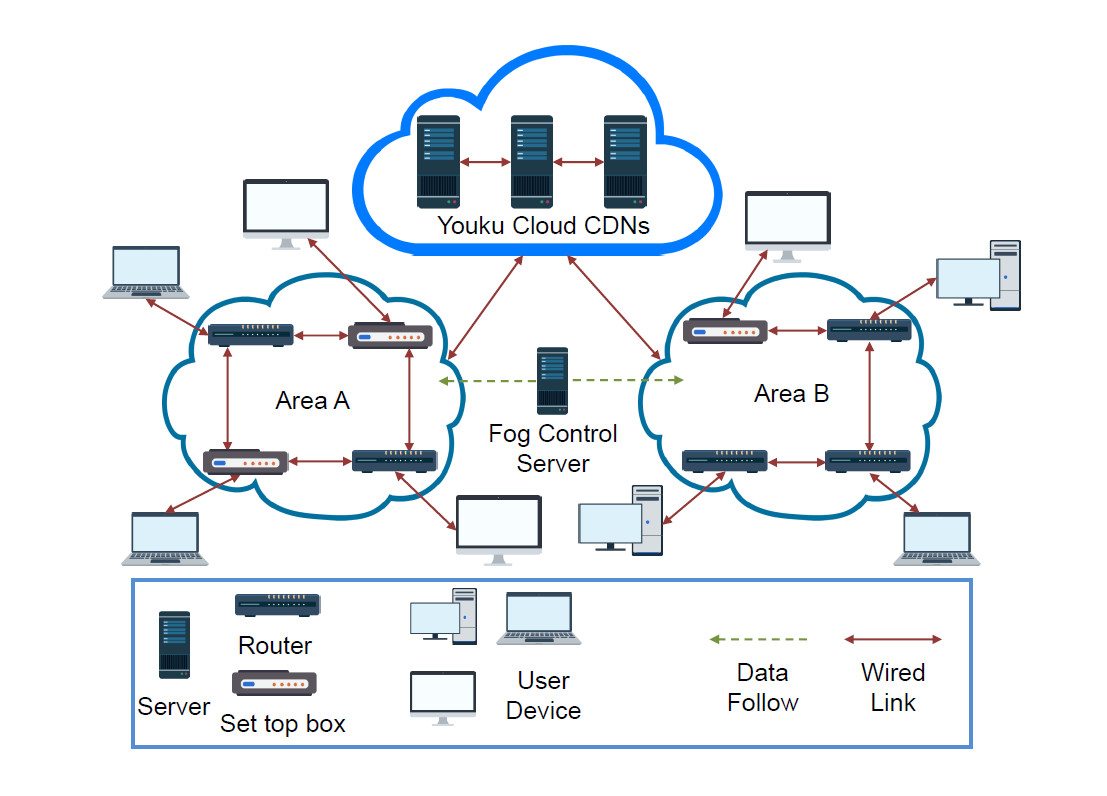
\includegraphics[width=\textwidth]{fig_4.png}
    \caption{Architecture of the peer CDN system of Youku}
 \label{fig_4}
\end{figure}


\subsection{Combing Replication with Recommendation}
\label{subsection_1}
Youku uses a centralized content replication strategy. Both the content push and content
removal are scheduled by the centralized control. Video popularity is the most critical
infuential factor in the video placement. The videos that are popular in the recent month are
likely to be replicated in smart-routers, e.g., over 60\% of the peer-videos are among 1200 most
popular videos of the recent month. Youku content replication strategy is insensitive to the
local content popularity and scheduled globally. However, Youku combines the replication
strategy with its recommendation system.

Video recommendation means the recommendation of videos by Youku, e.g., the homepage
 of Youku generally presents the newly published videos, recommended videos and popular
 video links, which can attract users to click. It is observed that 73\% of the videos
stored by our peer routers are on the homepage, and TV series and cartoon have the highest
possibility to be stored by smart-routers when they are recommended.

The downloaded chunk number follows a daily pattern, i.e., the lower levels of chunk
downloaded happen between 5 and 7 A.M. and 2 and 4 P.M. every day, and the peaks happen
between 0 and 3 A.M., which indicates that chunk downloading is scheduled periodically (i.e.,
hourly) during a day. It is likely that Youku makes replication decision on a daily basis and
push the contents during the time when the Internet traffic level is low.

\subsection{Centralized User Access Coordination}
\label{subsection_2}

The coordinating system in Youku is highly centralized. Youku has 4 kinds of servers to
manage the smart routers:
\begin{itemize}
	\item Config servers: Peer routers download configuration parameters from Config servers.
  \item QoS monitors: Peer routers report statistics to the QoS monitor server, including the
information of their partners and their operation states.
  \item Scheduling servers: Scheduling servers schedule the content replication according to the
information monitored.
  \item Agent managers: A set of agent managers is deployed in different ISPs and locations,
where each of them manages the smart-routers that are close to it.
\end{itemize}

As it seems that Youku do not care about the local content popularity, the control servers
can give similar instruction on all the fog devices. The fog devices usually store the similar
popular contents, so the users only need tond the nearest available fog device for the video
contents. The agent managers can make sure that users mostly request the content with the
same ISP domain.

\section{Thunder Crystal: Crowd-sourcing Content Distribution}

Thunder (Xunlei) is a popular P2P file sharing client side software in China \citep{Dhungel2011Measurement} \citep{Dhungel2012Xunlei}. To
extend their business, their users who have installed Thunder software (which are called
agents) can help some video content providers to distribute the content for monetary return.
The operator of Thunder Crystal, together with some researchers, has published some work
to illustrate how Thunder Crystal works \citep{Chen2015Thunder}.

In this work \citep{Chen2015Thunder} the Thunder Crystal is called a crowdsourcing system. In Thunder Crystal,
 Thunder asks some users (agents) with surplus bandwidth and computing resources to
support its content delivery. Unlike traditional P2P paradigm, Thunder's cloud servers have
the right to keep pushing content to agents if the agents agree to contribute their storage (to
store content) and upload bandwidth (to distribute content to end users) by rebated cash
from Thunder Crystal. Each agent is like a mini-CDN edge server, which is very close to end
users.

Most agents are normal Internet users who would like to offer their surplus bandwidth
with very low charge, but a user can have a better price by contributing their bandwidth in
peak hour. However, with the current price, it is enough for a user to cover its electricity
and network utility bills. Compared to the charging policies of the CDN companies, the
cash rebated to agents is much lower, implying lower expenses for distribution service. We
describe the approaches Thunder uses to deal with the major challenges on video replication
(Section \ref{subsection_3}) and access (Section \ref{subsection_4}) as follows.
\begin{figure}[htbp]
\centering
	  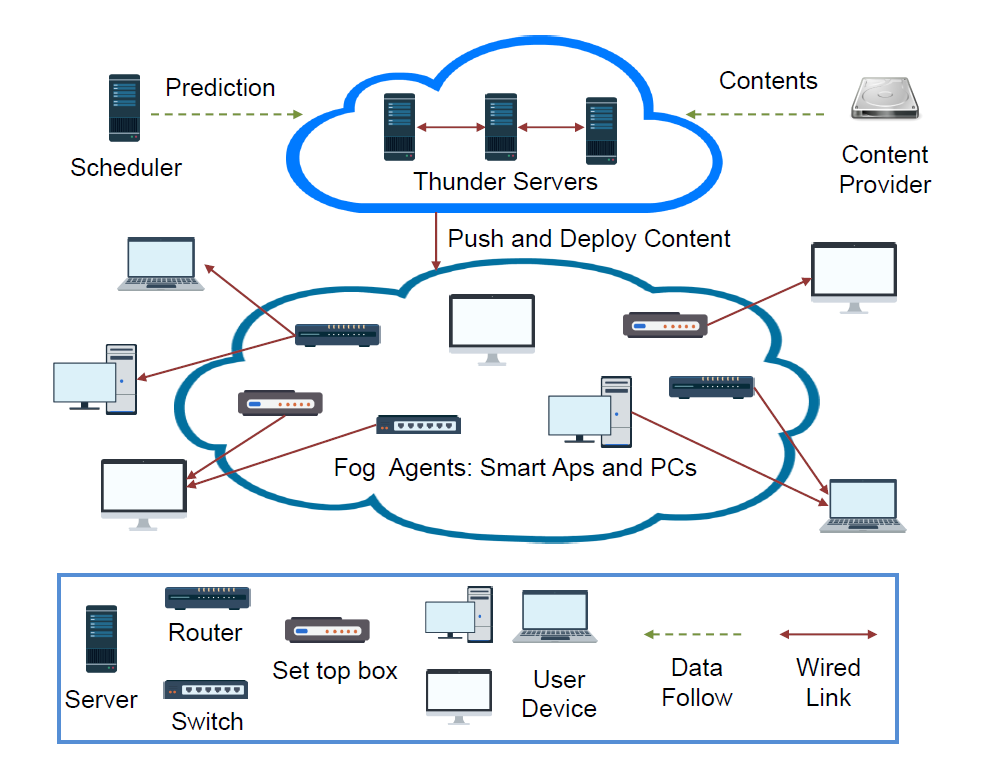
\includegraphics[width=\textwidth]{fig_5.png}
    \caption{System overview and general architecture of Thunder Crystal}
 \label{fig_5}
\end{figure}


\subsection{Replication Based on Popularity}
\label{subsection_3}
In Thunder's pushing strategy, agent devices are not discriminated. Thunder servers push
the new replicas randomly to different agent devices. Therefore, the fog network has no
locality awareness. Thunder servers can push 80TB traffic per day as their traffic budget.
Files will be pushed out by decreasing order of popularity until the traffic quota is used up.
In other words, more popularles will be pushed with higher priority than less popular files.
If the storage of an agent is full, thele with the lowest global popularity will be replaced.

To calculate the global popularity, besides the new contents, if the number of requests to
download a file is N, Thunder Crystal will maintain $ (0.05N)^{0.96}$ replications in the next day.
Such formula is obtained from experimental trials.

\subsection{Random User Access}
\label{subsection_4}
In current Thunder Crystal system, there are more than 11K active agent devices, which
is smaller than the scale of Youku. For each agent device, it serves all received requests
with best efforts. For each user, the file downloading is conducted chunk by chunk with
each chunk size 2MB. The first chunk is from the cloud CDN, and the rest of the chunks
will be chosen from around 200 agent devices with the desired content randomly. Therefore,
Thunder Crystal uses random video access scheme, which is not ISP friendly.

A data report module is embedded into the software that installed on the agent devices.
Reported information includes the number of agent devices that are working at any moment,
measured instant uploading speed, event-driven messages recording the access log of content
and other activities. To protect the copyright and avoid the user to falsely report its
contribution, all the files on any agent's fog device are encrypted.
